\begin{figure*}[!t]
\centering
\subfigure[Intent Detection] {
    \label{fig_overview_intent}
    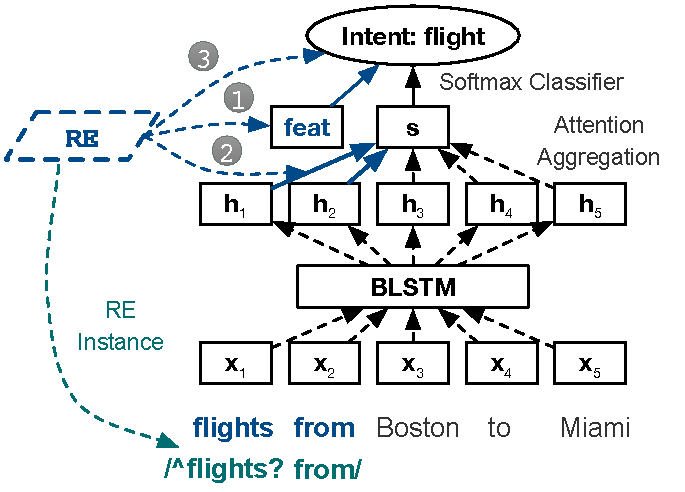
\includegraphics[width=0.8\columnwidth]{figure/re_nn_overview_intent.pdf}
}
\hspace{.5in}
\subfigure[Slot Filling (predicting slot label for \textsl{\underline{Boston}})] {
    \label{fig_overview_slot}
    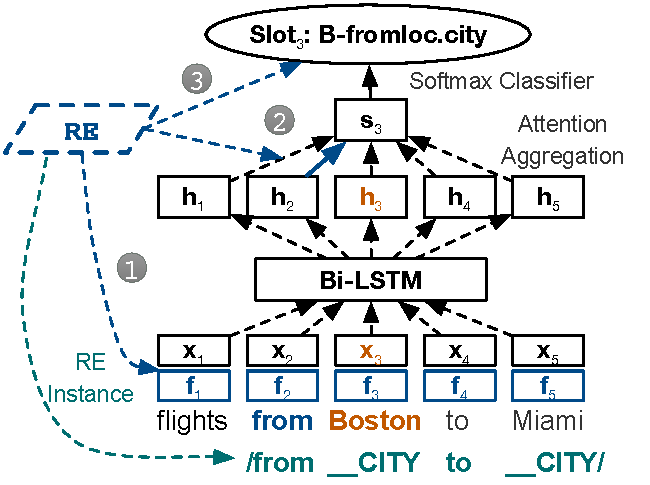
\includegraphics[width=0.8\columnwidth]{figure/re_nn_overview_slot.pdf}
}
\vspace{-3mm}
\caption{Overview of our methods. \circled{1}, \circled{2}, \circled{3} refers to the methods in
Sec.~\ref{fusion_with_input}, \ref{interact_with_module}, \ref{fusion_with_output} respectively.}
 % and the \RE that applies to the input
% sentence is shown in the bottom.}
\label{fig_overview}
\vspace{-5mm}
\end{figure*}

\section{Our Approach}
As depicted in Fig.~\ref{fig_overview}, we propose  to combine \NNs and \REs from three different angles.
 % for intent detection and slot filling.
% We present each method in the following sub-sections, starting by describing the base \NN model used by all the three methods.

\subsection{Base Models}
\label{sec:baseline} We use the Bi-directional LSTM (\BLSTM) as our base \NN model because it is effective in both intent detection and
slot filling~\cite{liu2016attention}.
% Further, to obtain sentence embedding for intent detection, we use a self-attention layer upon the \BLSTM output.

\cparagraph{Intent Detection} As shown in Fig.~\ref{fig_overview}, the \BLSTM takes as input the word embeddings $[\textbf{x}_1, ...,
\textbf{x}_n]$ of a n-word sentence, and produces a vector $\textbf{h}_i$ for each word $i$. A self-attention layer then takes in the
vectors produced by the \BLSTM to compute the sentence embedding $\textbf{s}$:
\begin{equation}
\textbf{s} = \sum_{i}{\alpha_i\textbf{h}_i}, \quad \alpha_i=\frac{\exp(\textbf{h}_i^\intercal \textbf{Wc})}{\sum_{i}{\exp(\textbf{h}_i^\intercal \textbf{Wc})}}
\label{eq:simple_att}
\end{equation}
where  $\alpha_i$ is the attention for word $i$, $\textbf{c}$ is a randomly initialized trainable vector used to select informative words for classification, and $\textbf{W}$ is a weight matrix.
Finally, $\textbf{s}$ is fed to a softmax classifier for intent classification.

\cparagraph{Slot Filling} The model for slot filling is  straightforward -- the slot label prediction is generated by a softmax classier
which takes in the \BLSTM's output $\textbf{h}_i$ and produces the slot label of word $i$. Note that attention aggregation in
Fig.~\ref{fig_overview} is only employed by the network module level method presented in Sec.~\ref{interact_with_module}.


\subsection{Using REs at the Input Level}
\label{fusion_with_input}
% Similar to the stacking technique \cite{wolpert1992stacked}, a straightforward way to combine \RE and \NN is to use the output of \RE patterns as feature, and feed them as input of \NN models.
At the input level, we use the evaluation outcomes of \REs as features which are fed to \NN models.

\cparagraph{Intent Detection}
Our \REtag for intent detection is the same as our target intent label.
% \footnote{If no \RE matches, we will assign a special tag indicating no matches. This process is applied to all the settings.}
Because real-world \REs are unlikely to be perfect, one sentence may be matched by more than one \RE. This may result in several \REtags
that are conflict with each other. For instance, the sentence \textsl{\underline{list the Delta airlines flights to Miami}} can match a
\RE: {\small \texttt{/list(\;the)?\;\_\_AIRLINE/}} that outputs tag \emph{airline}, and another \RE: {\small \texttt{/list(\,\textbackslash
w+)\{0,3\} flights?/}} that outputs tag \emph{flight}.
% \footnote{\texttt{\_\_WORD} matches a single word, which can be \texttt{/\textbackslash w+/}.}

To resolve the conflicting situations illustrated above, we average the randomly initialized trainable tag embeddings to form an aggregated
embedding as the \NN input. There are two ways to use the aggregated embedding. We can  append the aggregated embedding to either the
embedding of every input word, or the input of the softmax classifier (see \circled{1} in Fig.~\ref{fig_overview_intent}). To determine
which strategy works best, we perform a pilot study. We found that the first method causes the tag embedding to be copied many times;
consequently, the \NN tends to heavily rely on the \REtags, and the resulting performance is similar to the one given by using \REs alone
in few-shot settings. Thus, we adopt the second approach.
% In our pilot experiments on the
%first method, the tag embedding is copied so many times that tends to make the \NN heavily relies on the \REtags, making the performance
%similar to using \RE alone in few-shot settings. We therefore adopt the second method in this paper.

\cparagraph{Slot Filling} Since the evaluation outcomes of slot \REs are word-level tags,
we can simply embed and average the \REtags into a vector $\textbf{f}_i$ for each word, and append it
to the corresponding word embedding $\textbf{w}_i$ (as shown in \circled{1} in Fig.~\ref{fig_overview_slot}).
%Further, since our slot labels follow the \BIO annotation paradigm,
Note that we also extend the slot \REtags into the \BIO format, e.g., the \REtags of phrase \textsl{\underline{New York}} are \emph{B-city} and \emph{I-city} if its original tag is \emph{city}.

\subsection{Using REs at the Network Module Level}
\label{interact_with_module} At the network module level, we explore ways to utilize the clue words in the surface form of a \RE (bold blue arrows and
words in \circled{2} of Fig.~\ref{fig_overview}) to guide the attention module in \NNs.

%Since the \RE itself has already highlighted the clue words (bold blue arrows and words in \circled{2} of Fig.~\ref{fig_overview}) for its output tag, it can therefore help us guide the attention module in \NN.

\cparagraph{Intent Detection} Taking the sentence in Fig.~\ref{atis_sample} for example, the \RE: {\small\texttt{/\textasciicircum
flights?\:from/} } that leads to intent \emph{flight} means that \textsl{\underline{flights from}} are the key words to decide the intent
\emph{flight}. Therefore, the attention module in \NNs should leverage these two words to get the correct prediction. To this end, we
extend the base intent model by making two changes to incorporate the guidance from \REs.

First, since each intent has its own clue words, using a single sentence embedding for all intent labels %which is produced by only one set of attention,
would make the attention less focused.
% Considering we also know the intent that each \RE points to,
Therefore, we let each intent label $k$ use different attention $\textbf{a}_k$, which is then used to generate the sentence embedding
$\textbf{s}_k$ for that intent:
\begin{equation}
\textbf{s}_k = \sum_{i}{\alpha_{ki}\textbf{h}_i}, \quad
\alpha_{ki}=\frac{\exp(\textbf{h}_i^\intercal \textbf{W}_a\textbf{c}_k)}{\sum_{i}{\exp(\textbf{h}_i^\intercal \textbf{W}_a\textbf{c}_k)}}
\label{label_att_eq}
\end{equation}
where $\textbf{c}_k$ is a trainable vector for intent $k$ which is used to compute attention $\textbf{a}_k$, $\textbf{h}_i$ is the \BLSTM output for word $i$, and $\textbf{W}_a$ is a weight matrix.

The probability $p_k$ that the input sentence expresses intent $k$ is computed by:
\begin{equation}
p_k = \frac{\exp(logit_k)}{\sum_{k}{\exp(logit_k)}}, \quad\quad logit_k=\textbf{w}_k\textbf{s}_k + b_k
\label{label_prob_eq}
\end{equation}
where $\textbf{w}_k$, $logit_k$, $b_k$ are weight vector, logit, and bias for intent $k$, respectively.

Second, apart from indicating a sentence for intent $k$ (\textbf{\emph{positive \REs}}),
a \RE can also indicate that a sentence does not express intent $k$ (\textbf{\emph{negative \REs}}).
%Therefore, to make use of negative \REs,
We thus use a new set of attention (\textbf{\emph{negative attentions}}, in contrast to \textbf{\emph{positive attentions}}), to compute
another set of logits for each intent with Eqs.~\ref{label_att_eq} and \ref{label_prob_eq}. We denote the logits computed by positive
attentions as $logit_{pk}$, and those by negative attentions as $logit_{nk}$, the final logit for intent $k$ can then be calculated as:
\begin{equation}
logit_k = logit_{pk} - logit_{nk}
\end{equation}

To use \REs to guide attention, we add an attention loss to the final loss:
\begin{equation}
%loss_{att} = \sum_{k}{m_k\sum_{i}{t_{ki}\log(\alpha_{ki})}}
loss_{att} = \sum_{k}{\sum_{i}{t_{ki}\log(\alpha_{ki})}}
\label{att_loss}
\end{equation}
where $t_{ki}$ is set to $0$ when none of the matched \REs (that leads to intent $k$) marks word $i$ as a clue word -- otherwise $t_{ki}$
is set to $1/l_{k}$, where $l_k$ is the number of clue words
% mark by \RE
for intent $k$ (if no matched \RE leads to intent $k$, then $t_{k*}=0$).
%$m_k$ is a 0-1 indicator that is set to 1 when there is a matched \RE that leads to intent $k$.
We use Eq.~\ref{att_loss}
to compute the positive attention loss, $loss_{att\_p}$, for positive \REs and negative attention loss, $loss_{att\_n}$, for negative ones.
The final loss is computed as:
\begin{equation}
loss = loss_{c} + \beta_p loss_{att\_p} + \beta_n loss_{att\_n}
\end{equation}
where $loss_{c}$ is the original classification loss, $\beta_p$ and $\beta_n$ are weights for the two attention losses.

\cparagraph{Slot Filling}
%While we can apply the same \textbf{\emph{two-side attention}} (positive and negative attention) mechanism
%as we do in intent prediction, we will face an efficiency problem in slot filling.
The \textbf{\emph{two-side attention}} (positive and negative attention) mechanism introduced for intent prediction is unsuitable for slot
filling. Because for slot filling, we need to compute attention for each word, which demands more computational and memory resources than
doing that for intent detection\footnote{Since we need to assign a label to each word, if we still compute attention for each slot label,
we will have to compute $2\times L \times n^2$ attention values for one sentence. Here, $L$ is the number of tags and $n$ is the sentence
length. The \BIO tagging format will further double the number of tags.}.

Because of the aforementioned reason, we use a simplified version of the two-side attention, where all the slot labels share the same set
of positive and negative attention. Specifically, to predict the slot label of word $i$, we use the following equations, which are similar
to Eq.~\ref{eq:simple_att}, to generate a sentence embedding $\textbf{s}_{pi}$ with regard to word $i$ from positive attention:
\begin{equation}
\textbf{s}_{pi} = \sum_{j}{\alpha_{pij}\textbf{h}_j}, \quad \alpha_{pij}=\frac{exp(\textbf{h}_j^T\textbf{W}_{sp}\textbf{h}_i)}{\sum_{j}{exp(\textbf{h}_j^T\textbf{W}_{sp}\textbf{h}_i)}}
\label{eq:slu_simple_att}
\end{equation}
where $\textbf{h}_i$ and $\textbf{h}_j$ are the \BLSTM outputs for word $i$ and $j$ respectively, $\textbf{W}_{sp}$ is a weight matrix, and
$\alpha_{pij}$ is the positive attention value for word $j$ with respect to word $i$. Further, by replacing $\textbf{W}_{sp}$ with
$\textbf{W}_{sn}$, we use  Eq.~\ref{eq:slu_simple_att} again to compute negative attention and generate the corresponding sentence
embedding $\textbf{s}_{ni}$.

Finally, the prediction $\textbf{p}_i$ for word $i$ can be calculated as:
\begin{equation}
\begin{split}
\textbf{p}_i = \softmax((\textbf{W}_p [\textbf{s}_{pi}; \textbf{h}_i] + \textbf{b}_p) \\- (\textbf{W}_n [\textbf{s}_{ni}; \textbf{h}_i] + \textbf{b}_n))
\end{split}
\end{equation}
where $\textbf{W}_{p}$, $\textbf{W}_{n}$, $\textbf{b}_{p}$, $\textbf{b}_{n}$ are weight matrices and bias vectors for positive and negative attention, respectively. Here we append the \BLSTM output $\textbf{h}_i$ to $\textbf{s}_{pi}$ and $\textbf{s}_{ni}$ because the word $i$ itself also plays a crucial part in identifying its slot label.

\subsection{Using REs at the Output Level}
\label{fusion_with_output} At the output level, \REs are used to amend the output of \NNs. At this level, we take the same approach used
for intent detection and slot filling (see \circled{3} in Fig.~\ref{fig_overview}).

% Therefore, instead using a teach-student framework, this enables us to directly influence the logits of each label in a trainable way, so that we do not need to assign a weight for each pattern, and significantly reduces the number of hyper-parameters.

As mentioned in Sec.~\ref{re_desc}, the slot \REs used in the output level only produce a simplified version of target slot labels, for which
we can further
%Since the \REtag is related to the slot label, we can further
annotate their corresponding target slot labels.
% To make connections between the \RE tag and the slot label, we further annotate all the slot labels that the output tag may lead to.
For instance, a \RE that outputs \emph{city} can lead to three slot labels: \emph{fromloc.city}, \emph{toloc.city},
\emph{stoploc.city}.
% Actually, annotating this kind of connections is not difficult, since the \RE tags are generally somewhat related to the target label that we are trying to predict, otherwise the \RE tags will not be able to provide useful information for the prediction.

Let $z_k$ be a 0-1 indicator of whether there is at least one matched \RE that leads to target label $k$ (intent or slot label), the final
logits of label $k$ for a sentence (or a specific word for slot filling) is:
\begin{equation}
logit_k = logit'_k + w_k z_k
\end{equation}
where $logit'_k$ is the logit produced by the original \NN, and $w_k$ is a trainable weight indicating the overall confidence for \REs that
lead to target label $k$. Here we do not assign a trainable weight for each \RE because it is often that only a few sentences match a \RE.

We modify the logit instead of the final probability because a logit is an unconstrained real value, which matches the property of $w_k
z_k$ better than probability. Actually, when performing model ensemble,
% kagglers have also proved emperically that,
ensembling with logits is often empirically better than with the final probability\footnote{ An example can be found in the ensemble
version that Juan et al.~\shortcite{juan2016field} used in the Avazu Kaggle competition. }. This is also the reason why we choose to
operate on logits in Sec.~\ref{interact_with_module}.
